\section{Linear Filtering}

Filtering an image is a way to augment or extract information from it. Linear filters are a subset of operations that operate on a neighbourhood of pixels in an image. All linear filters operate on the same prinicpal, that is, they output a weighted average of their input. Filters take pixels in the neighbourhood covered by the filter as input. It is the weightings of a filter, known as filter coefficients, that determine the effect of the filter. These weights are stored in a matrix called a mask or kernel (see Figure \ref{fig:generalForm}) that's then convolved or correlated with an image (see sections \ref{subsection:corr} \& \ref{subsection:conv}).


\begin{figure}[h]
  
   \[ 
     Kernel  = \frac{1}{\sum\limits_{i=0}^{M}\sum\limits_{j=0}^{N}c_{i,j}}
    \begin{bmatrix}
      c_{0,0} & c_{0,1} & \dots & c_{0,n} \\
      c_{1,0} & c_{1,1} & \dots & c_{1,n} \\
      \vdots & \vdots & \ddots & \vdots \\
      c_{m,0} & c_{m,1} & \dots & c_{m,n}
    \end{bmatrix}
  \]
  \caption{General Form of a Linear Filter}
  \label{fig:generalForm}
\end{figure}

 A filter kernel is nearly always square so as to have a center cell which sits atop a reference pixel. The result of the filter's application at that reference pixel will be stored in the output image at the location of the reference pixel. Notice in Figure \ref{fig:kernel_graphics} how the mask sits over the reference pixel.

% TREE %
\begin{figure}[H]
  \centering
  \centering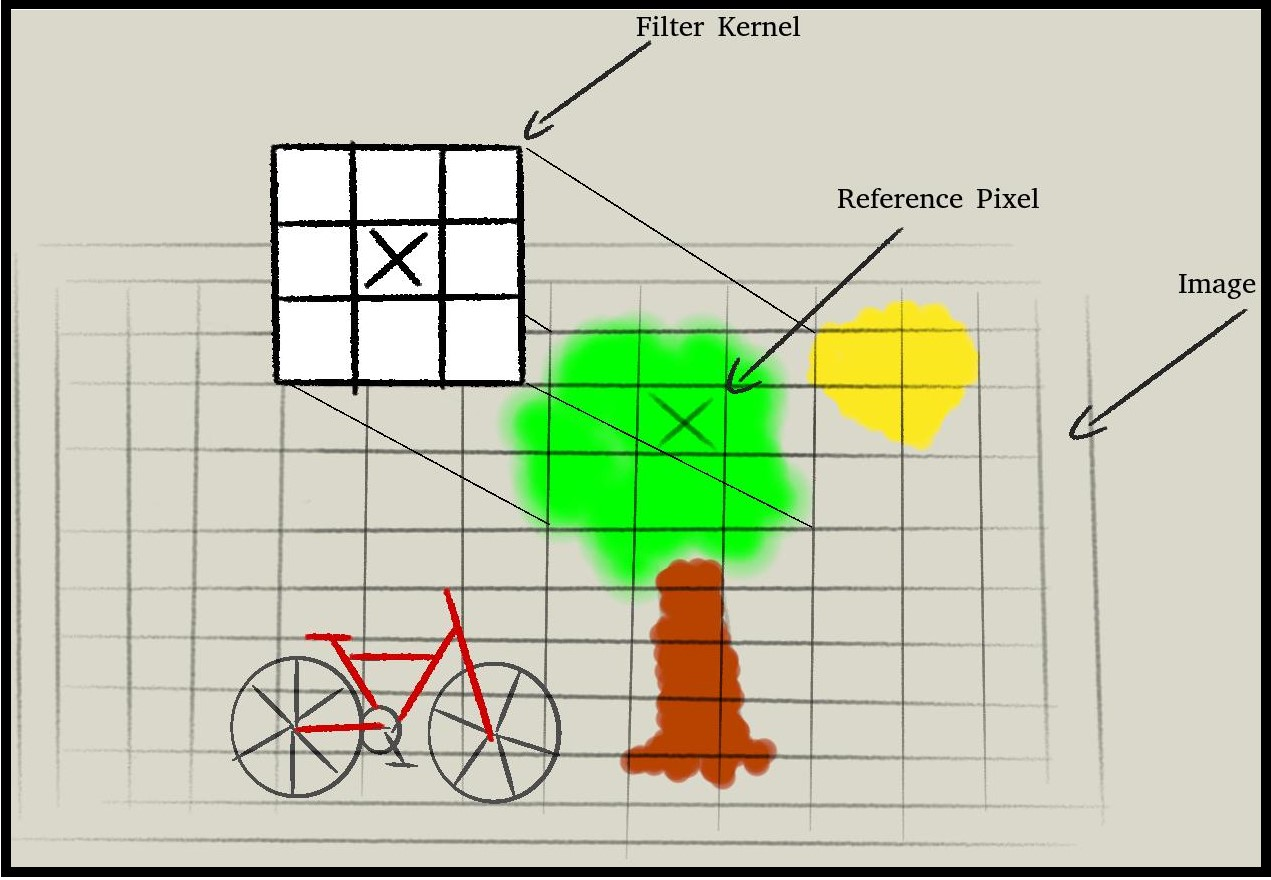
\includegraphics[width=350pt]{kernel_graphics}
  \caption{Visualization of a Filter Kernel Application}
  \label{fig:kernel_graphics}
\end{figure}

A 'box filter', for example, outputs the average of its inputs because the filter weights are evenly distributed. By passing this filter over an image its sharpness is reduced giving a smoothing or blurring effect. This can be observed in Figure \ref{fig:roughDog}.

% DOG BOX FILTERED%
\begin{figure}[H]
  \centering
  \begin{subfigure}[b]{0.75\textwidth}
    \centering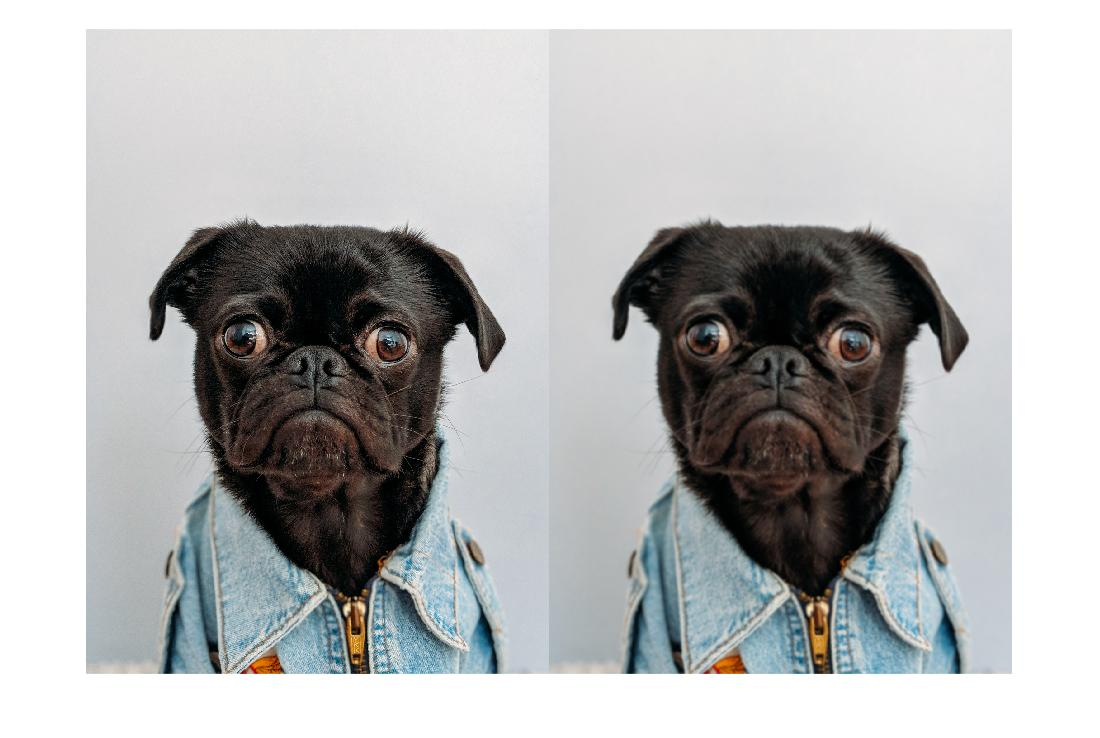
\includegraphics[width=300pt]{dogPug}
    \caption{Left: Photo by Charles Deluvio. Right: Application of $16\times16$ box filter.}
    \label{fig:roughDog}
  \end{subfigure}
  \begin{subfigure}[b]{0.25\textwidth}
    \centering
    \[
      \frac{1}{9}
    \begin{bmatrix}
       1 & 1 & 1 \\
       1 & 1 & 1 \\
       1 & 1 & 1
    \end{bmatrix}
    \]
    \caption{Box Filter Kernel.}
    \label{fig:boxkernel}
  \end{subfigure}
  \caption{Box Filter application and kernel.}
  \label{fig:boxfilter}
\end{figure}

% CORRELATION
\subsection{Correlation}
\label{subsection:corr}
The application of a linear filter $h(u,v)$ to an image $f(i,j)$ may be described as follows

\begin{equation} \label{eq:1}
g(i,j) = \sum_{u=-k}^{k}\sum_{v = -l}^{l}f(i+u,j+v)h(u,v)
\end{equation}

$g(i,j)$ is the output image. Performing correlation with a filter may be notated more concisely by the correlation operator.

\[g = f \otimes h\]

Correlation measures the similarity between two signals. Both digital images and linear filters are two dimensional signals. Performing correlation between them will yield an output image where the highest values correspond to where the image and filter were most similar \cite{optimalKernel}. This useful because if you wish to emphasise a feature in an image it can be done by correlating it with a filter that describes that feature. For example, if you wished to exagerate vertical and horizontal lines you could use Sobel filters as in \ref{fig:sobel_filters}. 

% SOBEL MASKS
\begin{figure}[H]
  \begin{subfigure}[b]{0.49\textwidth}
    \[
    \begin{bmatrix*}[l]
     -1 & -1 & -1 \\
      \phantom{-}2 & \phantom{-}2 & \phantom{-}2 \\
      -1 & -1 & -1 
    \end{bmatrix*}
    \]
    \caption{Horizontal Sobel Filter Mask}
    \label{rfidtest_xaxis}
\end{subfigure}
\begin{subfigure}[b]{0.49\textwidth}
  \[ 
    \begin{bmatrix}
      -1 & 2 & -1 \\
      -1 & 2 & -1 \\
      -1 & 2 & -1
    \end{bmatrix}
    \]
    \caption{Vertical Sobel Filter Mask}  
\end{subfigure}
    \caption{Sobel Filters}
    \label{fig:sobel_filters}
\end{figure}

The use of negative weightings means that values next to an edge are diminished and the positively weighted line sections (the 2s) strengthen line features. Notice in figure \ref{fig:sobel_apply} how the lines have a high values (white) and regions that aren't lines are low valued (black).

% SOBEL FILTER APPLICATION
\begin{figure}[H]
  \centering
  \begin{subfigure}[b]{0.3\textwidth}
      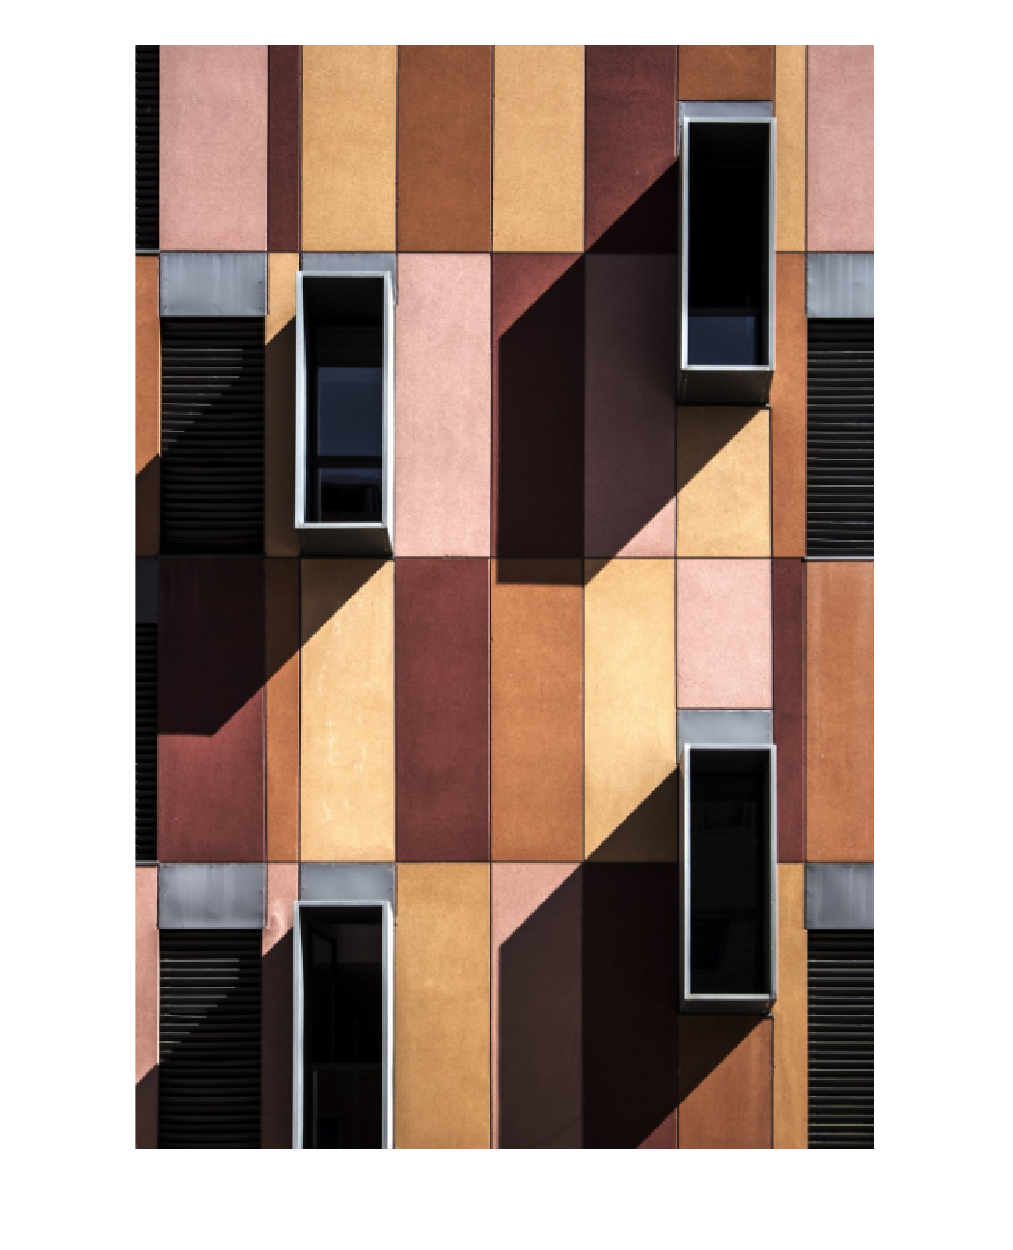
\includegraphics[width=\textwidth]{im_color}
      \caption{Image by Simone Hutsch}
  \end{subfigure}
  \begin{subfigure}[b]{0.3\textwidth}
      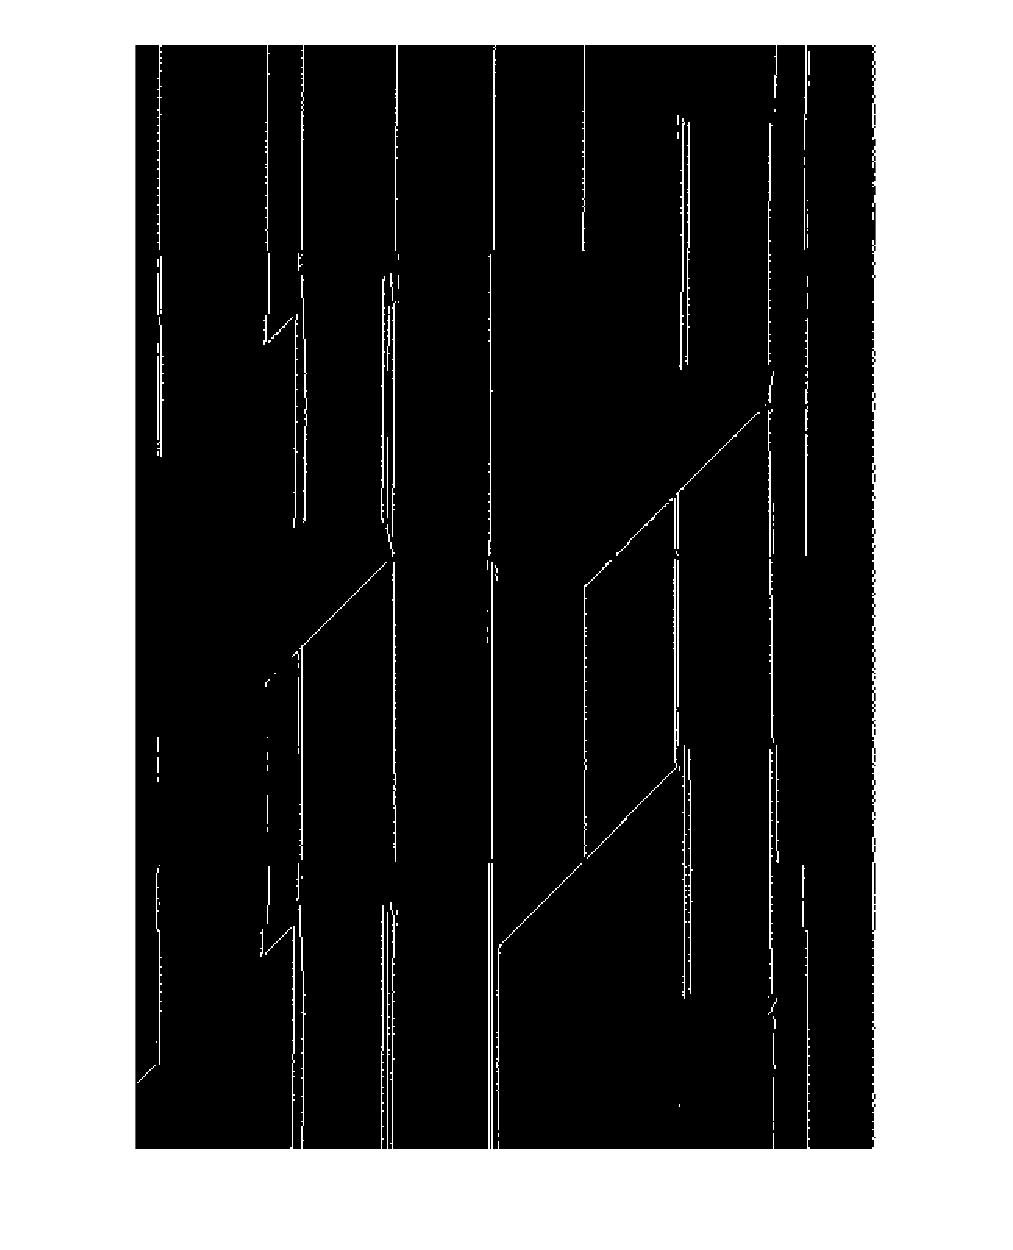
\includegraphics[width=\textwidth]{gv}
      \caption{Vertical Sobel Filter}
      \label{fig:vert}
  \end{subfigure}
  \begin{subfigure}[b]{0.3\textwidth}
      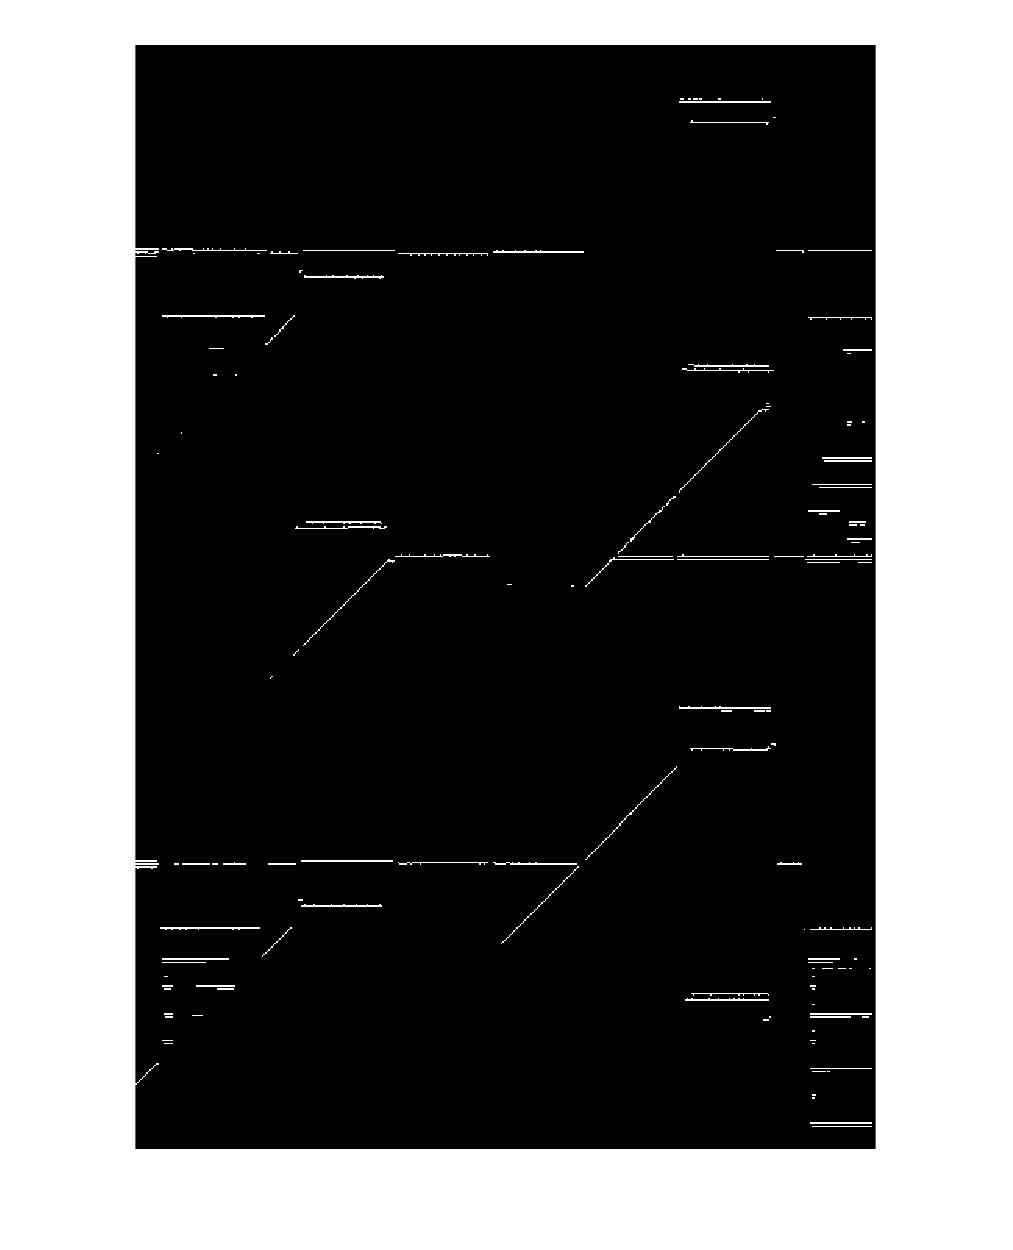
\includegraphics[width=\textwidth]{gh}
      \caption{Horizontal Sobel Filter}
      \label{fig:hoz}
  \end{subfigure}
  \caption{Application of Sobel filters to exagerate lines.}
  \label{fig:sobel_apply}
\end{figure}

Correlation is \emph{shift invariant}, which means that it does the same thing no matter where in an image it is applied. To satisfy this property correlation may be superpositioned 

\[a(f_1 + f_2) = af_1 + af_2\]

and abides by the shift invariance principle

\[g(i,j)=f(i+k,j+l) \Leftrightarrow\ (h\circ g)(i,j)=(h\circ f)(i+k,j+l)\]

Correlation has the side effect of flipping both horizontally and vertically the location of output points relative to location the center point (\emph{reference point}) in the original image which may be undesirable.

% CORRELATION EXAMPLE  %
\begin{figure}[H] 
  \centering
  \begin{tabular}{ccccc}
      \begin{tabular}{|c|c|c|c|c|}
      \hline
      0 & 0 & 0 & 0 & 0 \\[1pt]
      \hline
      0 & 0 & 0 & 0 & 0 \\[1pt]
      \hline
      0 & 0 & 1 & 0 & 0 \\[1pt]
      \hline
      0 & 0 & 0 & 0 & 0 \\[1pt]
      \hline
      0 & 0 & 0 & 0 & 0 \\[1pt]
      \hline
      \end{tabular}%
    & $\otimes$ &
    \begin{tabular}{|c|c|c|}
      \hline
      a & b & c \\
      \hline
      d & e & f \\
      \hline
      g & h & i \\
      \hline 
    \end{tabular}
    & $=$ &
    \begin{tabular}{|c|c|c|c|c|}
      \hline
      0 & 0 & 0 & 0 & 0 \\[1pt]
      \hline
      0 & \textbf{i} & \textbf{h} & \textbf{g} & 0 \\[1pt]
      \hline
      0 & \textbf{f} & \textbf{e} & \textbf{d} & 0 \\[1pt]
      \hline
      0 & \textbf{c} & \textbf{b} & \textbf{a} & 0 \\[1pt]
      \hline
      0 & 0 & 0 & 0 & 0 \\[1pt]
      \hline
    \end{tabular} \\
    $F(x,y)$ & & $H(u,v)$& & $G(x,y)$ \\
  \end{tabular}
  \caption{Correlation of a filter and an image.}
  \label{fig:correlation}
\end{figure}


\subsection{Convolution}
\label{subsection:conv}
Convolution is also a linear operation that is shift invariant. It is very similar to correlation except that where correlation measure similarity between signals convolution measures the effect of one signal on another. It is described mathematically by the expression,

\[ g(i,j) = \sum_{u=-k}^{k}\sum_{v = -l}^{l}f(u,v)h(i-u,j-v)\]

Notice that the filter $h(i,j)$ is rotated  180 degrees. This causes the output's orientation to match the original image. Convolution may be notated as follows,

\[g = f \ast h\]

% Convolution example  %
\begin{figure}[H] 
  \centering
  \begin{tabular}{ccccc}
      \begin{tabular}{|c|c|c|c|c|}
      \hline
      0 & 0 & 0 & 0 & 0 \\[1pt]
      \hline
      0 & 0 & 0 & 0 & 0 \\[1pt]
      \hline
      0 & 0 & 1 & 0 & 0 \\[1pt]
      \hline
      0 & 0 & 0 & 0 & 0 \\[1pt]
      \hline
      0 & 0 & 0 & 0 & 0 \\[1pt]
      \hline
      \end{tabular}%
    & $\ast$ &
    \begin{tabular}{|c|c|c|}
      \hline
      a & b & c \\
      \hline
      d & e & f \\
      \hline
      g & h & i \\
      \hline 
    \end{tabular}
    & $=$ &
    \begin{tabular}{|c|c|c|c|c|}
      \hline
      0 & 0 & 0 & 0 & 0 \\[1pt]
      \hline
      0 &  \textbf{a} & \textbf{b} & \textbf{c} & 0 \\[1pt]
      \hline
      0 & \textbf{d} & \textbf{e} & \textbf{f} & 0 \\[1pt]
      \hline
      0 & \textbf{g} & \textbf{h} & \textbf{i} & 0 \\[1pt]
      \hline
      0 & 0 & 0 & 0 & 0 \\[1pt]
      \hline
    \end{tabular} \\
    $F(x,y)$ & & $H(u,v)$& & $G(x,y)$ \\
  \end{tabular}
  \caption{Convolution of a filter and an image.}
  \label{fig:convolution}
\end{figure}